\documentclass{beamer}

% Top-aligning columns within a top-aligned frame
% https://tex.stackexchange.com/questions/16447/beamer-top-aligning-columns-within-a-top-aligned-frame
\makeatletter
\newenvironment{myitemize}{%
   \setlength{\topsep}{0pt}
   \setlength{\partopsep}{0pt}
   \renewcommand*{\@listi}{\leftmargin\leftmargini \parsep\z@ \topsep\z@ \itemsep\z@}
   \let\@listI\@listi
   \itemize
}{\enditemize}
\makeatother  

\usepackage[USenglish]{babel}
\usepackage[utf8]{inputenc}
\usepackage{amssymb, amsmath}
\usepackage{bm}
\usepackage{color}
\usepackage{tikz}
\usepackage{url}

\definecolor{links}{HTML}{2A1B81}
\hypersetup{colorlinks,linkcolor=,urlcolor=links}

\usetheme{Boadilla}
\setbeamertemplate{headline}{}
\newcommand*\oldmacro{}%
\let\oldmacro\insertshorttitle%
\renewcommand*\insertshorttitle{%
  \oldmacro\hfill%
  \insertframenumber\,/\,\inserttotalframenumber}
  

\bibliographystyle{apalike}
% make bibliography entries smaller
%\renewcommand\bibfont{\scriptsize}
% Now get rid of all the colours
\setbeamercolor*{bibliography entry title}{fg=black}
\setbeamercolor*{bibliography entry author}{fg=black}
\setbeamercolor*{bibliography entry location}{fg=black}
\setbeamercolor*{bibliography entry note}{fg=black}

% and kill the abominable icon
\setbeamertemplate{bibliography item}{}

\begin{document}
\title{Dataset Distillation}  
\author{Radek Bartyzal}
\date{13. 12. 2018} 
\institute{Let's talk ML in Prague}

\frame{\titlepage} 
%--------- END Frame 1 -------------

\begin{frame}[t]{Knowledge distillation}

\begin{columns}[t]
\begin{column}{0.5\textwidth}
Teacher
\begin{itemize}
\item high-capacity model
\item good performance
\end{itemize}
\end{column}

\begin{column}{0.5\textwidth}
Student
\begin{itemize}
\item more compact model
\item not as good performance as the teacher but better than if it was trained without it
\end{itemize}
\end{column}

\end{columns}

\vfill
By transferring knowledge, one hopes to benefit from the student’s
compactness while suffering only minimal degradation in performance \cite{cit:anc}, \cite{cit:distill}.

\end{frame}
%--------- END Frame 9 -------------
\begin{frame}{Dataset Distillation}

\begin{enumerate}
\item pick an original dataset e.g. MNIST
\item select a specific architecture and initial weights
\item synthesize new smaller dataset using the selected architecture and weights
\item train the model on this small dataset
\item evaluate the model on the test set of the original dataset
\end{enumerate}

\end{frame}
%--------- END Frame 9 -------------
\begin{frame}{Problems}

\textbf{Problem:}\\
Why not just remember the final trained weights instead of the initial ones?

\vfill

\textbf{Solution:}
\begin{itemize}
\item init weights are from a distribution D
\item create such examples that work for multiple sampled init weights
\end{itemize}

\end{frame}
%--------- END Frame 9 -------------
\begin{frame}{Uses}

\textbf{Advantages:}
\begin{itemize}
\item compressed representation
\item faster training - only couple GD steps\
\item fine-tune pre-trained weights to new dataset
\item dataset poisoning = fine-tune the model to predict trash
\item how much can we compress the information of the dataset?
\item can we train the model by synthetic images that
are not on the natural image manifold?
\end{itemize}

\vfill

\textbf{Compressed representation:}
\begin{itemize}
\item architecture
\item init weights distribution
\item learned learning rate
\item created small train dataset
\end{itemize}

\end{frame}
%--------- END Frame 9 -------------
\begin{frame}{Algorithm}
\begin{figure}[h]
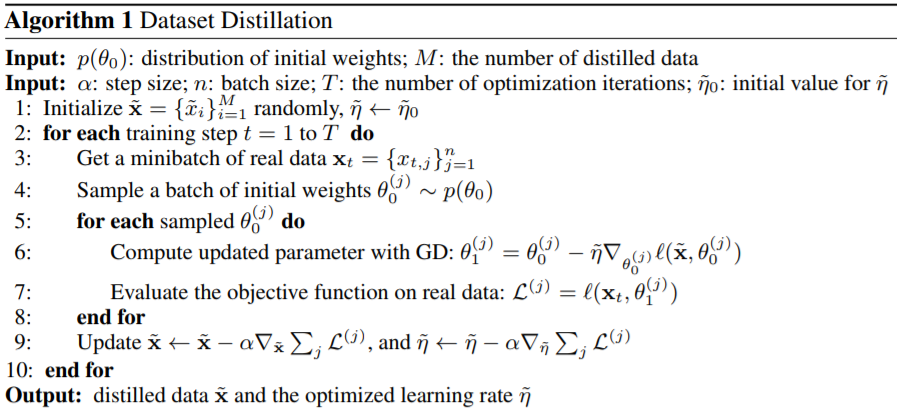
\includegraphics[width=\textwidth]{img/alg1}
%\caption{ \cite{cit:resnet}}
\end{figure}
\end{frame}

%--------- END Frame 9 -------------
\begin{frame}{Results}
\begin{figure}[h]
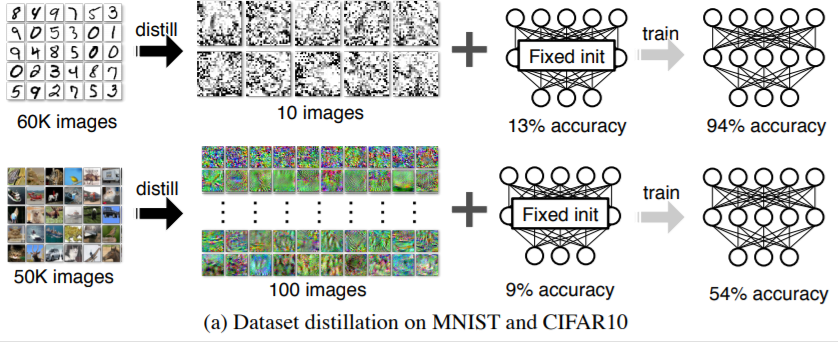
\includegraphics[width=\textwidth]{img/uses1}
\caption{Fixed = sampled from }
\end{figure}
\end{frame}
%--------- END Frame 9 -------------
\begin{frame}{Results}
\begin{figure}[h]
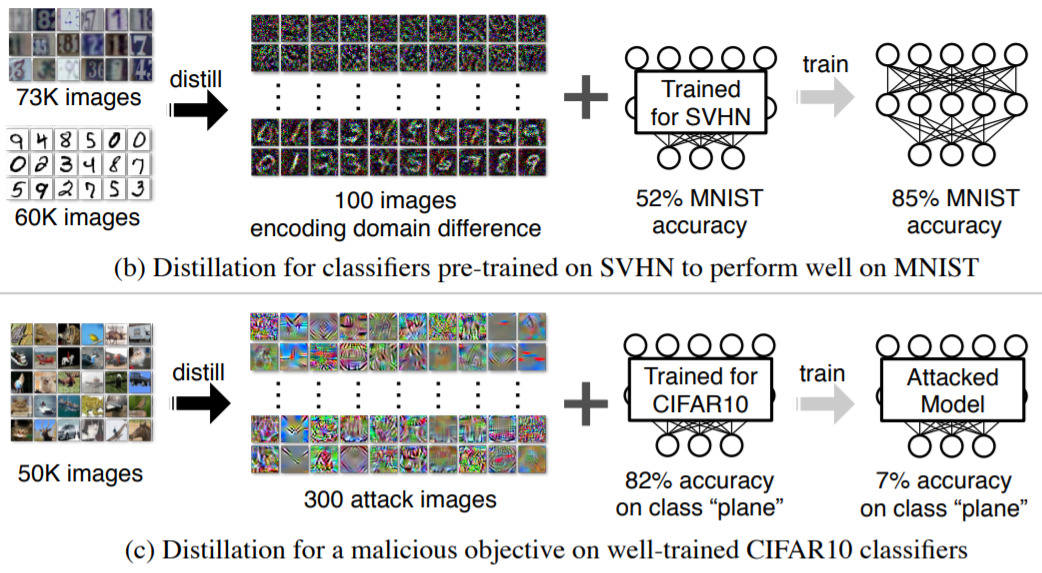
\includegraphics[width=\textwidth]{img/uses2}
%\caption{ \cite{cit:resnet}}
\end{figure}
\end{frame}
%--------- END Frame 9 -------------
\begin{frame}{Results}
\begin{figure}[h]
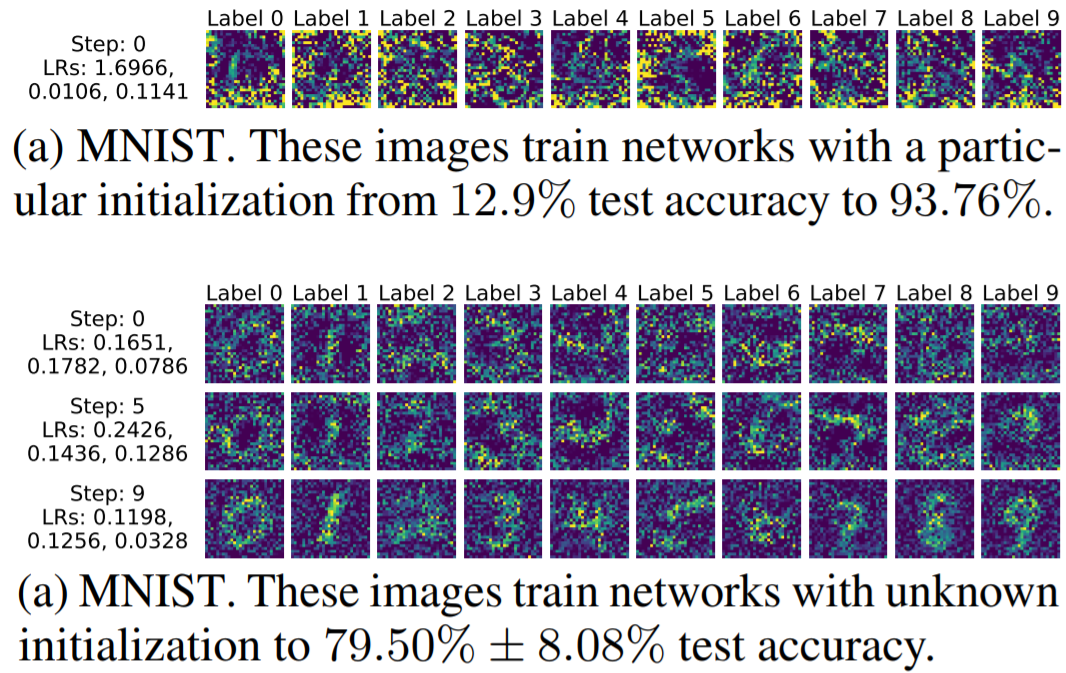
\includegraphics[width=\textwidth]{img/results1}
%\caption{Fixed = sampled from }
\end{figure}
\end{frame}
%--------- END Frame 9 -------------
\begin{frame}{Results}
\begin{figure}[h]
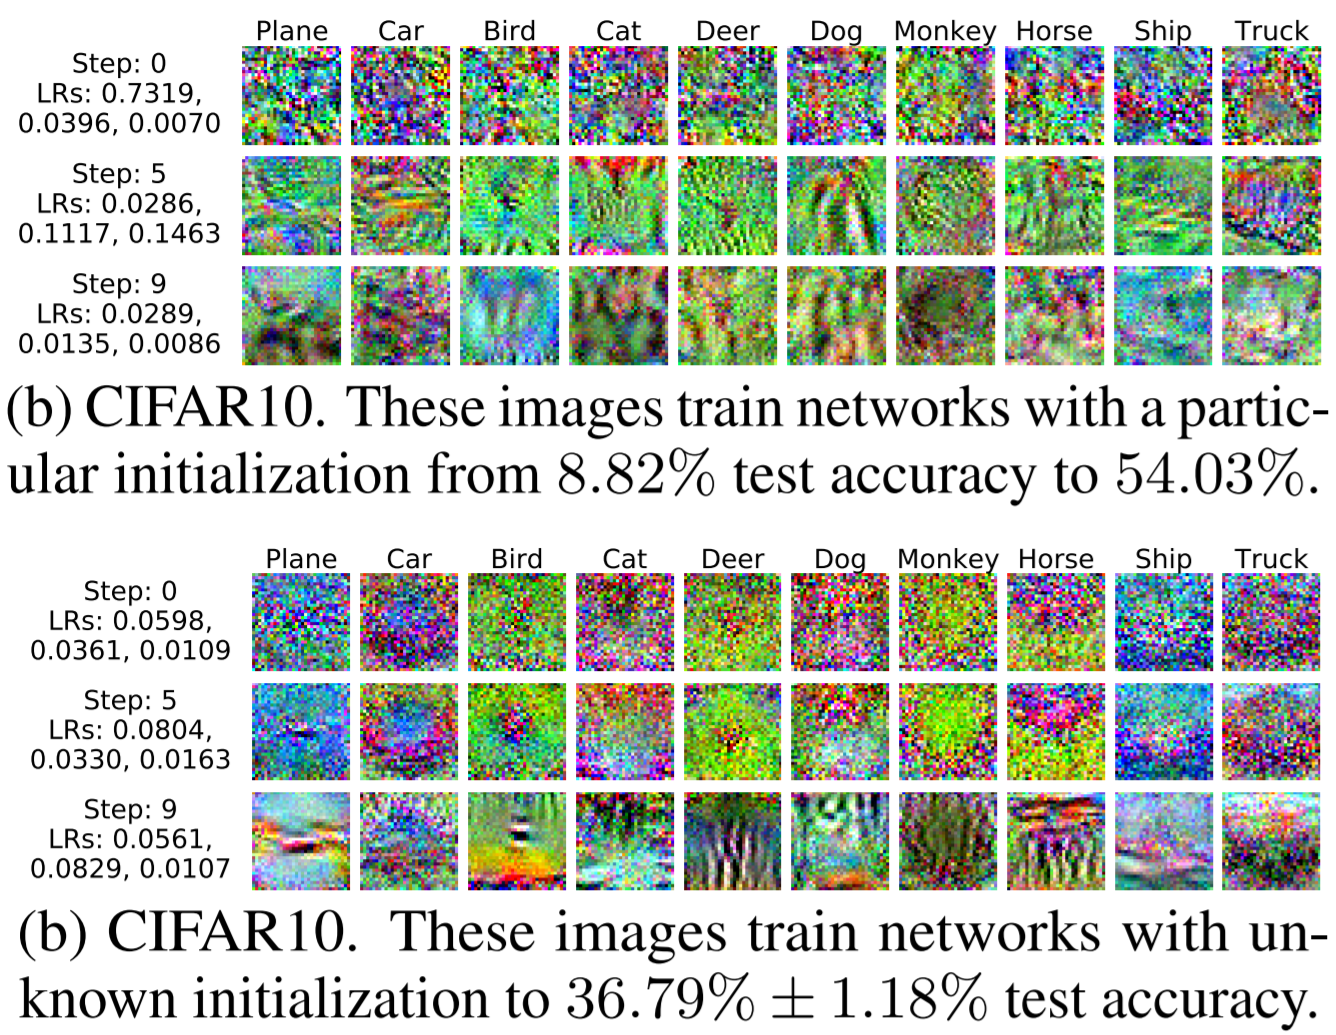
\includegraphics[width=0.85\textwidth]{img/results2}
%\caption{ \cite{cit:resnet}}
\end{figure}
\end{frame}
%--------- END Frame 12 -------------
\begin{frame}{Sources}

\begin{thebibliography}{0}

  \bibitem[1]{cit:anc} 1. Belagiannis, Vasileios, Azade Farshad, and Fabio Galasso. "Adversarial Network Compression." arXiv preprint arXiv:1803.10750 (2018). Accessible from: \url{https://arxiv.org/abs/1803.10750}
  
  \bibitem[2]{cit:dd} 2. Wang, Tongzhou, et al. "Dataset Distillation." Arxiv preprint. 2018. Accessible from: \url{https://arxiv.org/abs/1811.10959v1}
  
  
\end{thebibliography}

\end{frame}


\begin{frame}{Sources}

\begin{thebibliography}{0}
  \bibitem[3]{cit:bat} 4. Breiman, Leo, and Nong Shang. "Born again trees." ps (1996). Accessible from: \url{https://www.stat.berkeley.edu/~breiman/BAtrees.pdf}
  
  \bibitem[4]{cit:distill} 5. Hinton, Geoffrey, Oriol Vinyals, and Jeff Dean. "Distilling the knowledge in a neural network." arXiv preprint arXiv:1503.02531 (2015). Accessible from: \url{https://arxiv.org/pdf/1503.02531.pdf}
  

\end{thebibliography}

\end{frame}
 
 
 
\end{document}
